% !TEX root = ../Thesis.tex
\myChapter{The mammalian lung}\label{ch:lung}
\begin{flushright}{\slshape I'm throwing rocks tonight. Mark it, Dude.} \\ \medskip
    --- \defcitealias{TheBigLebowski}{Steve Buscemi as Donny}\citetalias{TheBigLebowski} \citep{TheBigLebowski}
\end{flushright}
\bigskip
\section{Interestingness}
Why is the mammalian lung so interesting?

\section{Lung Development}
During lung development all the internal structures like the conducting airways, the blood vessel network and the gas exchange area are formed. The lung is specifically designed to provide this large gas exchange surface---in humans the alveolar gas exchange surface is in the order of \SI{130}{\meter\squared}, an area equivalent to about $\frac{3}{4}$ of a tennis court~\cite{Weibel2009}---where capillary blood efficiently gets in close contact to the air inside the lung structure. 

Mammalian lung development can be divided into five overlapping stages~\cite{Schittny2004}, as shown in figure~\ref{fig:lung development stages}: Organogenesis starts with a outpouching of the foregut resulting in the appearance of the lung buds. Subsequently, the conducting and parts of the respiratory airways are formed by a successive cycle of branching and growth starting at the lung buds, which is called branching morphogenesis. Most of this process takes place during the pseudoglandular stage.

\begin{figure}[htb]
	\centering
	\pgfplotsset{width=\linewidth,height=.5\linewidth}
	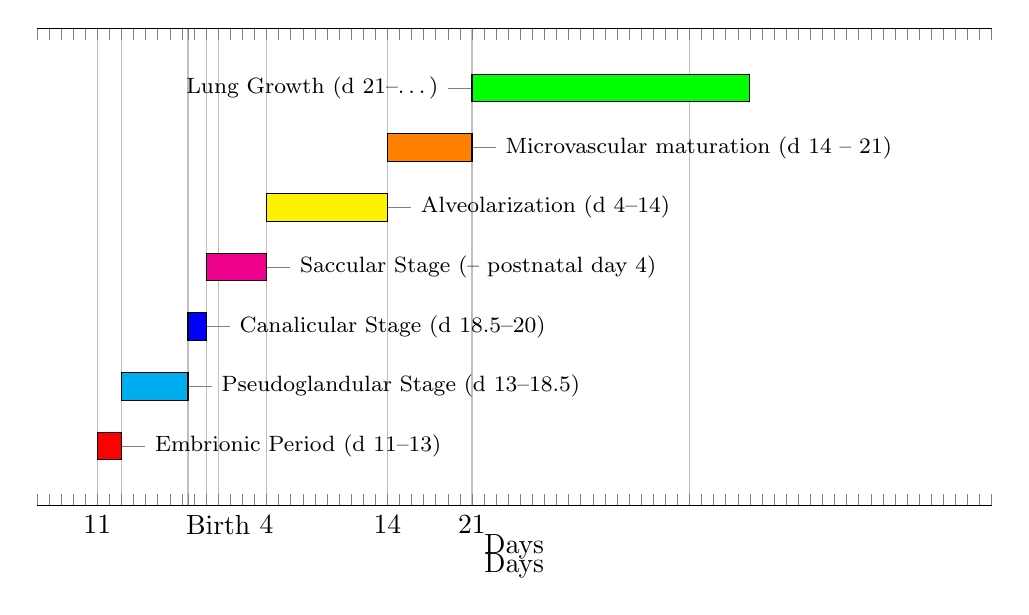
\begin{tikzpicture}
		\begin{axis}[xbar stacked,%
			scale only axis,%
			xmin=6,%
			xmax=85,%
			ymin=0,%
			ymax=0.4,%
			yticklabels={},%
			xtick={1,...,85},%
			xticklabels={},
			xlabel=Days,%
			axis y line=none]
		\end{axis}
		\begin{axis}[xbar stacked,%
			scale only axis,%
			xmin=6,%
			xmax=85,%
			ymin=0,%
			ymax=0.4,%
			yticklabels={},%
			xtick={11,13,18.5,20,21,25,35,42,60},%
			xticklabels={11,,,,Birth,4,14,21},
			xmajorgrids,%
			xlabel=Days,%
			%axis x line=bottom,%
			axis y line=none]
			\def\step{0.05}
			\addplot [transparent] coordinates {(11,0)};
			\addplot [fill=red] coordinates {(2,1*\step)};
			\addplot [fill=cyan] coordinates {(5.5,2*\step)};
			\addplot [fill=blue] coordinates {(1.5,3*\step)};
			\addplot [fill=magenta] coordinates {(5,4*\step)};
			\addplot [fill=yellow] coordinates {(10,5*\step)};
			\addplot [fill=orange] coordinates {(7,6*\step)};
			\addplot [fill=green] coordinates {(23,7*\step)};

			\tikzstyle{every pin}=[%
				%fill=white,%
				%semitransparent,%
				%draw=black,%
				% text width=20em,%
				font=\footnotesize,
				text centered,%
				pin distance=2ex]
			\node[coordinate, pin=right:{Embrionic Period (d 11--13)}] at (axis cs:13,0.05) {};
			\node[coordinate, pin=right:{Pseudoglandular Stage (d 13--18.5)}] at (axis cs:18.5,0.1) {};
			\node[coordinate, pin=right:{Canalicular Stage (d 18.5--20)}] at (axis cs:20,0.15) {};
			\node[coordinate, pin=right:{Saccular Stage (-- postnatal day 4)}] at (axis cs:25,0.2) {};
			\node[coordinate, pin=right:{Alveolarization (d 4--14)}] at (axis cs:35,0.25) {};
			\node[coordinate, pin=right:{Microvascular maturation (d 14 -- 21)}] at (axis cs:42,0.3) {};
			\node[coordinate, pin=left:{Lung Growth (d 21--\dots)}] at (axis cs:42,0.35) {};
		\end{axis}
	\end{tikzpicture}
	\caption{Lung development stages for the rat lung (modified from \ldots). The first three stages (Embrionic Period, Pseudoglandular and Canalicular Stage) take place in the approximately 21 days from the beginning of gestation to birth. The stages are partially overlapping, which is not shown in this figure.}
	\todo[inline]{Reference? really Rat?}
	\label{fig:lung development stages}
\end{figure}

This stage is followed by intermediate stages, which are called ca\-na\-li\-cular and saccular. During the canalicular stage a first functional gas exchange surface---the air-blood barrier---is formed. The saccular stage marks the switch from branching to septation morphogenesis.

During the alveolar stage the distal part of the bronchial tree is enlarged by a lifting off of additional septa from already existing septa (septation/alveolarization). 

In order to optimize gas exchange after bulk alveolarization is completed, the interalveolar septa and their capillary networks are remodeled during the phase of microvascular maturation. At this point lung development is considered as being finished and normal growth of the organ follows.

The time point of birth differs between mammals, relative to the state of lung development. In humans, birth happens at the beginning of the alveolar stage.

It was believed that lung developments comes to completion during the early postnatal period due to the reduction of a double- to a single-layered capillaries network inside the alveolar septa (microvasculature maturation postnatal days 14–-21 in rats). After this period, only growth of the organ should follow, and no more alveolar septa are built in the lung~\cite{Burri1999,Schittny2004}. \citet{Schittny2008} were able to show that so called late alveolarization happens, where alveolar septa are are formed until young adulthood (days 4–-60 in rats). A local duplication of the capillary network was detected as the basis of these newly forming septa.